%!TEX program = xelatex
\documentclass[a4paper,11pt]{article}
\usepackage{kotex}
\usepackage{amsmath,amssymb}
\usepackage{geometry}
\usepackage{multicol}
\usepackage{array}
\usepackage{tabularx}
\usepackage{booktabs}
\usepackage{enumitem}
\usepackage{tikz}
\usepackage{xcolor}
\usepackage{mdframed}

\geometry{top=15mm, bottom=15mm, left=15mm, right=15mm}

\setmainfont{NanumMyeongjo}
\setsansfont{NanumGothic}

\setlength{\columnseprule}{0.4pt}
\setlength{\columnsep}{8mm}

\newcommand{\choicenum}[1]{\textcircled{\small #1}}
\newcommand{\scorebox}[1]{\textbf{(#1점)}}
\newcommand{\qbox}[1]{%
  \begin{mdframed}[linewidth=0.8pt,innerleftmargin=6pt,innerrightmargin=6pt,innertopmargin=4pt,innerbottommargin=4pt]
  #1
  \end{mdframed}
}

\pagestyle{empty}

\begin{document}

%--- 헤더 ---
\begin{center}
{\large \textbf{3학년 1학기 중간고사 \quad 수학 \quad [A형]}}\\[2pt]
{\normalsize 선택형 1번\,--\,16번 \;/\; 서술형 1번\,--\,8번 \quad 총 4쪽}
\end{center}
\vspace{1mm}
\hrule height 1pt
\vspace{3mm}

\begin{multicols}{2}

%===========================================================
%  선택형
%===========================================================

\noindent\textbf{1.} $\sqrt{(-5)^{2}}$의 제곱근은? \scorebox{3}

\begin{enumerate}[label=\protect\choicenum{\arabic*},leftmargin=*,itemsep=0pt]
  \item $\pm\,5$
  \item $\pm\,\sqrt{5}$
  \item $5$
  \item $-5$
  \item $25$
\end{enumerate}

\vspace{3mm}

\noindent\textbf{2.} 실수의 대소관계로 옳은 것은? \scorebox{3}

\begin{enumerate}[label=\protect\choicenum{\arabic*},leftmargin=*,itemsep=0pt]
  \item $\sqrt{30} > 6$
  \item $\sqrt{5} < 2$
  \item $-\sqrt{20} > -5$
  \item $-\sqrt{15} < -4$
  \item $\dfrac{\sqrt{5}}{4} > \dfrac{\sqrt{7}}{4}$
\end{enumerate}

\vspace{3mm}

\noindent\textbf{3.} 다음을 계산하면? \scorebox{3}

\qbox{$\sqrt{32} \div \sqrt{8} \times 2\sqrt{3}$}

\begin{enumerate}[label=\protect\choicenum{\arabic*},leftmargin=*,itemsep=0pt]
  \item $2\sqrt{3}$
  \item $4\sqrt{3}$
  \item $6\sqrt{3}$
  \item $8\sqrt{3}$
  \item $12\sqrt{3}$
\end{enumerate}

\vspace{3mm}

\noindent\textbf{4.} 다음 식을 전개하면? \scorebox{3}

\qbox{$(3x+2y)(3x-2y)$}

\begin{enumerate}[label=\protect\choicenum{\arabic*},leftmargin=*,itemsep=0pt]
  \item $3x^{2}-2y^{2}$
  \item $9x^{2}-4y^{2}$
  \item $3x^{2}-4y^{2}$
  \item $9x^{2}+12xy-4y^{2}$
  \item $9x^{2}-12xy+4y^{2}$
\end{enumerate}

\vspace{3mm}

\noindent\textbf{5.} 다음 식이 완전제곱식이 되도록\\
\quad $\square$ 안에 알맞은 수를 고르면? \scorebox{3}

\qbox{$4x^{2}-20x+\square$}

\begin{enumerate}[label=\protect\choicenum{\arabic*},leftmargin=*,itemsep=0pt]
  \item $4$
  \item $10$
  \item $16$
  \item $25$
  \item $100$
\end{enumerate}

\vspace{3mm}

\noindent\textbf{6.} 다음 이차방정식을 풀면? \scorebox{3}

\qbox{$x^{2}+8x=0$}

\begin{enumerate}[label=\protect\choicenum{\arabic*},leftmargin=*,itemsep=0pt]
  \item $x=-4$
  \item $x=-4$ 또는 $x=8$
  \item $x=0$ 또는 $x=-8$
  \item $x=0$ 또는 $x=8$
  \item $x=4$ 또는 $x=-8$
\end{enumerate}

\vspace{3mm}

\noindent\textbf{7.} 무리수만으로 짝지어진 것을 고르면? \scorebox{4}

\begin{enumerate}[label=\protect\choicenum{\arabic*},leftmargin=*,itemsep=0pt]
  \item $\sqrt{3},\,\sqrt{9},\,\sqrt{15}$
  \item $\sqrt{\dfrac{4}{9}},\,\sqrt{0.01},\,\pi$
  \item $0.8,\,\dfrac{16}{25},\,\sqrt{4}$
  \item $2\sqrt{3},\,3\sqrt{5},\,-\sqrt{0.09}$
  \item $\sqrt{1.44},\,-\sqrt{(-3)^{2}},\,\sqrt{16}-1$
\end{enumerate}

\vspace{3mm}

\noindent\textbf{8.} $0<x<1$일 때, 가장 큰 것을 고르면? \scorebox{4}

\begin{enumerate}[label=\protect\choicenum{\arabic*},leftmargin=*,itemsep=0pt]
  \item $\sqrt{x}$
  \item $x$
  \item $x^{2}$
  \item $\dfrac{1}{x}$
  \item $2x$
\end{enumerate}

\vspace{3mm}

\noindent\textbf{9.} 다음을 계산하면? \scorebox{4}

\qbox{$\sqrt{48}-\sqrt{27}+\sqrt{75}$}

\begin{enumerate}[label=\protect\choicenum{\arabic*},leftmargin=*,itemsep=0pt]
  \item $2\sqrt{3}$
  \item $3\sqrt{3}$
  \item $4\sqrt{3}$
  \item $5\sqrt{3}$
  \item $6\sqrt{3}$
\end{enumerate}

\vspace{3mm}

\noindent\textbf{10.} $\sqrt{12}\!\left(\dfrac{\sqrt{3}}{2}-\sqrt{3}\right)+\dfrac{a}{\sqrt{3}}\!\left(\sqrt{48}-2\right)$이\\
유리수일 때, 유리수 $a$의 값을 구하면? \scorebox{4}

\begin{enumerate}[label=\protect\choicenum{\arabic*},leftmargin=*,itemsep=0pt]
  \item $\dfrac{3}{4}$
  \item $\dfrac{3}{2}$
  \item $2$
  \item $3$
  \item $-2$
\end{enumerate}

\vspace{3mm}

\noindent\textbf{11.} 식을 전개할 때, $x$의 계수가 다른 하나는? \scorebox{4}

\begin{enumerate}[label=\protect\choicenum{\arabic*},leftmargin=*,itemsep=0pt]
  \item $(x+4)(x-5)$
  \item $(x+6)(-x+5)$
  \item $(x+2)(3x-4)$
  \item $(3x+2)(4x-1)$
  \item $(3x+4)(2x-5)$
\end{enumerate}

\vspace{3mm}

\noindent\textbf{12.} 다음 식을 전개하면? \scorebox{4}

\qbox{$(x+4y)^{2}-9\!\left(\dfrac{1}{3}x+y\right)^{2}$}

\begin{enumerate}[label=\protect\choicenum{\arabic*},leftmargin=*,itemsep=0pt]
  \item $-2xy-7y^{2}$
  \item $-4xy-5y^{2}$
  \item $2x^{2}+8xy+5y^{2}$
  \item $7xy+5y^{2}$
  \item $-3x^{2}-2xy-55y^{2}$
\end{enumerate}

\vspace{3mm}

\noindent\textbf{13.} 다음 두 다항식을 인수분해 할 때, 공통으로 들어 있는 인수는? \scorebox{4}

\qbox{$-(x-3)+2x(x-3),\quad 6x^{2}+x-2$}

\begin{enumerate}[label=\protect\choicenum{\arabic*},leftmargin=*,itemsep=0pt]
  \item $x-3$
  \item $2x-1$
  \item $2x+1$
  \item $3x+2$
  \item $3x-2$
\end{enumerate}

\vspace{3mm}

\noindent\textbf{14.} 다음 그림과 같은 직사각형의 빗금친 부분의 넓이를 구하면? \scorebox{4}

\begin{center}
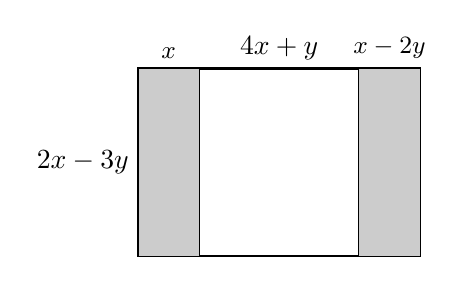
\begin{tikzpicture}[scale=0.85]
  \draw[thick] (0,0) rectangle (4.2,2.8);
  \draw[thick] (0.9,0) rectangle (3.3,2.8);
  \fill[gray!40] (0,0) rectangle (0.9,2.8);
  \fill[gray!40] (3.3,0) rectangle (4.2,2.8);
  \node at (2.1,3.1) {$4x+y$};
  \node at (-0.1,1.4) [rotate=90] {};
  \node[above] at (0.45,2.8) {\small $x$};
  \node[above] at (3.75,2.8) {\small $x-2y$};
  \node[left] at (0,1.4) {$2x-3y$};
\end{tikzpicture}
\end{center}

\begin{enumerate}[label=\protect\choicenum{\arabic*},leftmargin=*,itemsep=0pt]
  \item $6x^{2}-10xy-13y^{2}$
  \item $7x^{2}-14xy-9y^{2}$
  \item $8x^{2}-14xy+9y^{2}$
  \item $10x^{2}-28xy+7y^{2}$
  \item $11x^{2}-32xy+11y^{2}$
\end{enumerate}

\vspace{3mm}

\noindent\textbf{15.} $-4<x<\dfrac{1}{3}$일 때, 다음 식을 간단히 하면? \scorebox{5}

\qbox{$\sqrt{25+10x+x^{2}}-\sqrt{9x^{2}-6x+1}$}

\begin{enumerate}[label=\protect\choicenum{\arabic*},leftmargin=*,itemsep=0pt]
  \item $-x+6$
  \item $x-4$
  \item $2x-3$
  \item $3x+4$
  \item $4x+4$
\end{enumerate}

\vspace{3mm}

\noindent\textbf{16.} 두 자연수 $a,\,b$에 대하여 다항식 $3x^{2}+13x+k$가\\
$(3x+a)(x+b)$로 인수분해 되도록 하는 실수 $k$의\\
최댓값은? \scorebox{5}

\begin{enumerate}[label=\protect\choicenum{\arabic*},leftmargin=*,itemsep=0pt]
  \item $4$
  \item $10$
  \item $12$
  \item $14$
  \item $36$
\end{enumerate}

\end{multicols}

\newpage

%===========================================================
%  서술형
%===========================================================
\begin{center}
{\large \textbf{서술형 \quad [A형]}}
\end{center}
\noindent{\small ※ 서술형 문항은 \textbf{서술형 답지}에 풀이과정과 답을 쓰고 제출해야 합니다.}
\vspace{4mm}
\hrule
\vspace{4mm}

\begin{enumerate}[leftmargin=*,itemsep=10mm]

\item[\textbf{서술형 1.}] $\dfrac{\sqrt{5}+3}{\sqrt{5}}$의 분모를 유리화하여라. \scorebox{4}

\vspace{30mm}

\item[\textbf{서술형 2.}] 다음 식을 전개하여라. \scorebox{4}

\qbox{$(4x+1)^{2}-3x(x+2)$}

\vspace{35mm}

\item[\textbf{서술형 3.}] 다음 이차방정식을 인수분해를 이용하여 풀어라. \scorebox{5}

\qbox{$3x^{2}-10x-8=0$}

\vspace{35mm}

\item[\textbf{서술형 4.}] $\sqrt{\dfrac{700}{x}}$이 자연수가 되도록 하는 자연수 $x$의 값을 모두 구하여라. \scorebox{5}

\vspace{35mm}

\item[\textbf{서술형 5.}] 이차식 $ax^{2}-5x-6$, $3x^{2}+bx+4$의\\
공통인수가 $x-2$일 때, $a+b$의 값을 구하여라. \scorebox{5}

\vspace{35mm}

\item[\textbf{서술형 6.}] $-4^{2}+6^{2}-8^{2}+10^{2}-12^{2}+14^{2}$을\\
인수분해를 이용하여 계산하여라. \scorebox{5}

\vspace{35mm}

\item[\textbf{서술형 7.}] 다음 두 부등식을 모두 만족시키는 자연수 $x$의\\
값을 모두 더하면? \scorebox{6}

\qbox{%
\begin{tabular}{l}
① $\sqrt{28} < 2\sqrt{x} < \sqrt{60}$ \\[4pt]
② $-6 < -\sqrt{4x} < -4$
\end{tabular}
}

\vspace{40mm}

\item[\textbf{서술형 8.}] 사다리꼴 $ABDE$의 넓이를 구하고, 이것이\\
직사각형 $ACDF$의 넓이의 몇 배인지 구하여라. \scorebox{6}

\begin{center}
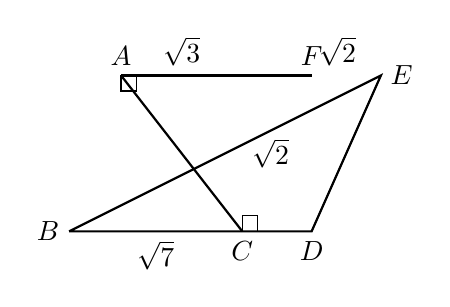
\begin{tikzpicture}[scale=1.1]
  \coordinate (B) at (0,0);
  \coordinate (C) at (2,0);
  \coordinate (D) at (2.8,0);
  \coordinate (A) at (0.6,1.8);
  \coordinate (E) at (3.6,1.8);
  \coordinate (F) at (2.8,1.8);
  \draw[thick] (B)--(E)--(D)--(B);
  \draw[thick] (A)--(F);
  \draw[thick] (C)--(A);
  \draw (A) rectangle ++(0.18,-0.18);
  \draw (C) rectangle ++(0.18,0.18);
  \node[left] at (B) {$B$};
  \node[below] at (C) {$C$};
  \node[below] at (D) {$D$};
  \node[above] at (A) {$A$};
  \node[right] at (E) {$E$};
  \node[above] at (F) {$F$};
  \node[below] at (1,0) {$\sqrt{7}$};
  \node[right] at (2,0.9) {$\sqrt{2}$};
  \node[above] at (1.3,1.8) {$\sqrt{3}$};
  \node[above] at (3.1,1.8) {$\sqrt{2}$};
\end{tikzpicture}
\end{center}

\end{enumerate}

\end{document}
